
% Default to the notebook output style

    


% Inherit from the specified cell style.




    
\documentclass[11pt]{article}

    
    
    \usepackage[T1]{fontenc}
    % Nicer default font (+ math font) than Computer Modern for most use cases
    \usepackage{mathpazo}

    % Basic figure setup, for now with no caption control since it's done
    % automatically by Pandoc (which extracts ![](path) syntax from Markdown).
    \usepackage{graphicx}
    % We will generate all images so they have a width \maxwidth. This means
    % that they will get their normal width if they fit onto the page, but
    % are scaled down if they would overflow the margins.
    \makeatletter
    \def\maxwidth{\ifdim\Gin@nat@width>\linewidth\linewidth
    \else\Gin@nat@width\fi}
    \makeatother
    \let\Oldincludegraphics\includegraphics
    % Set max figure width to be 80% of text width, for now hardcoded.
    \renewcommand{\includegraphics}[1]{\Oldincludegraphics[width=.8\maxwidth]{#1}}
    % Ensure that by default, figures have no caption (until we provide a
    % proper Figure object with a Caption API and a way to capture that
    % in the conversion process - todo).
    \usepackage{caption}
    \DeclareCaptionLabelFormat{nolabel}{}
    \captionsetup{labelformat=nolabel}

    \usepackage{adjustbox} % Used to constrain images to a maximum size 
    \usepackage{xcolor} % Allow colors to be defined
    \usepackage{enumerate} % Needed for markdown enumerations to work
    \usepackage{geometry} % Used to adjust the document margins
    \usepackage{amsmath} % Equations
    \usepackage{amssymb} % Equations
    \usepackage{textcomp} % defines textquotesingle
    % Hack from http://tex.stackexchange.com/a/47451/13684:
    \AtBeginDocument{%
        \def\PYZsq{\textquotesingle}% Upright quotes in Pygmentized code
    }
    \usepackage{upquote} % Upright quotes for verbatim code
    \usepackage{eurosym} % defines \euro
    \usepackage[mathletters]{ucs} % Extended unicode (utf-8) support
    \usepackage[utf8x]{inputenc} % Allow utf-8 characters in the tex document
    \usepackage{fancyvrb} % verbatim replacement that allows latex
    \usepackage{grffile} % extends the file name processing of package graphics 
                         % to support a larger range 
    % The hyperref package gives us a pdf with properly built
    % internal navigation ('pdf bookmarks' for the table of contents,
    % internal cross-reference links, web links for URLs, etc.)
    \usepackage{hyperref}
    \usepackage{longtable} % longtable support required by pandoc >1.10
    \usepackage{booktabs}  % table support for pandoc > 1.12.2
    \usepackage[inline]{enumitem} % IRkernel/repr support (it uses the enumerate* environment)
    \usepackage[normalem]{ulem} % ulem is needed to support strikethroughs (\sout)
                                % normalem makes italics be italics, not underlines
    

    
    
    % Colors for the hyperref package
    \definecolor{urlcolor}{rgb}{0,.145,.698}
    \definecolor{linkcolor}{rgb}{.71,0.21,0.01}
    \definecolor{citecolor}{rgb}{.12,.54,.11}

    % ANSI colors
    \definecolor{ansi-black}{HTML}{3E424D}
    \definecolor{ansi-black-intense}{HTML}{282C36}
    \definecolor{ansi-red}{HTML}{E75C58}
    \definecolor{ansi-red-intense}{HTML}{B22B31}
    \definecolor{ansi-green}{HTML}{00A250}
    \definecolor{ansi-green-intense}{HTML}{007427}
    \definecolor{ansi-yellow}{HTML}{DDB62B}
    \definecolor{ansi-yellow-intense}{HTML}{B27D12}
    \definecolor{ansi-blue}{HTML}{208FFB}
    \definecolor{ansi-blue-intense}{HTML}{0065CA}
    \definecolor{ansi-magenta}{HTML}{D160C4}
    \definecolor{ansi-magenta-intense}{HTML}{A03196}
    \definecolor{ansi-cyan}{HTML}{60C6C8}
    \definecolor{ansi-cyan-intense}{HTML}{258F8F}
    \definecolor{ansi-white}{HTML}{C5C1B4}
    \definecolor{ansi-white-intense}{HTML}{A1A6B2}

    % commands and environments needed by pandoc snippets
    % extracted from the output of `pandoc -s`
    \providecommand{\tightlist}{%
      \setlength{\itemsep}{0pt}\setlength{\parskip}{0pt}}
    \DefineVerbatimEnvironment{Highlighting}{Verbatim}{commandchars=\\\{\}}
    % Add ',fontsize=\small' for more characters per line
    \newenvironment{Shaded}{}{}
    \newcommand{\KeywordTok}[1]{\textcolor[rgb]{0.00,0.44,0.13}{\textbf{{#1}}}}
    \newcommand{\DataTypeTok}[1]{\textcolor[rgb]{0.56,0.13,0.00}{{#1}}}
    \newcommand{\DecValTok}[1]{\textcolor[rgb]{0.25,0.63,0.44}{{#1}}}
    \newcommand{\BaseNTok}[1]{\textcolor[rgb]{0.25,0.63,0.44}{{#1}}}
    \newcommand{\FloatTok}[1]{\textcolor[rgb]{0.25,0.63,0.44}{{#1}}}
    \newcommand{\CharTok}[1]{\textcolor[rgb]{0.25,0.44,0.63}{{#1}}}
    \newcommand{\StringTok}[1]{\textcolor[rgb]{0.25,0.44,0.63}{{#1}}}
    \newcommand{\CommentTok}[1]{\textcolor[rgb]{0.38,0.63,0.69}{\textit{{#1}}}}
    \newcommand{\OtherTok}[1]{\textcolor[rgb]{0.00,0.44,0.13}{{#1}}}
    \newcommand{\AlertTok}[1]{\textcolor[rgb]{1.00,0.00,0.00}{\textbf{{#1}}}}
    \newcommand{\FunctionTok}[1]{\textcolor[rgb]{0.02,0.16,0.49}{{#1}}}
    \newcommand{\RegionMarkerTok}[1]{{#1}}
    \newcommand{\ErrorTok}[1]{\textcolor[rgb]{1.00,0.00,0.00}{\textbf{{#1}}}}
    \newcommand{\NormalTok}[1]{{#1}}
    
    % Additional commands for more recent versions of Pandoc
    \newcommand{\ConstantTok}[1]{\textcolor[rgb]{0.53,0.00,0.00}{{#1}}}
    \newcommand{\SpecialCharTok}[1]{\textcolor[rgb]{0.25,0.44,0.63}{{#1}}}
    \newcommand{\VerbatimStringTok}[1]{\textcolor[rgb]{0.25,0.44,0.63}{{#1}}}
    \newcommand{\SpecialStringTok}[1]{\textcolor[rgb]{0.73,0.40,0.53}{{#1}}}
    \newcommand{\ImportTok}[1]{{#1}}
    \newcommand{\DocumentationTok}[1]{\textcolor[rgb]{0.73,0.13,0.13}{\textit{{#1}}}}
    \newcommand{\AnnotationTok}[1]{\textcolor[rgb]{0.38,0.63,0.69}{\textbf{\textit{{#1}}}}}
    \newcommand{\CommentVarTok}[1]{\textcolor[rgb]{0.38,0.63,0.69}{\textbf{\textit{{#1}}}}}
    \newcommand{\VariableTok}[1]{\textcolor[rgb]{0.10,0.09,0.49}{{#1}}}
    \newcommand{\ControlFlowTok}[1]{\textcolor[rgb]{0.00,0.44,0.13}{\textbf{{#1}}}}
    \newcommand{\OperatorTok}[1]{\textcolor[rgb]{0.40,0.40,0.40}{{#1}}}
    \newcommand{\BuiltInTok}[1]{{#1}}
    \newcommand{\ExtensionTok}[1]{{#1}}
    \newcommand{\PreprocessorTok}[1]{\textcolor[rgb]{0.74,0.48,0.00}{{#1}}}
    \newcommand{\AttributeTok}[1]{\textcolor[rgb]{0.49,0.56,0.16}{{#1}}}
    \newcommand{\InformationTok}[1]{\textcolor[rgb]{0.38,0.63,0.69}{\textbf{\textit{{#1}}}}}
    \newcommand{\WarningTok}[1]{\textcolor[rgb]{0.38,0.63,0.69}{\textbf{\textit{{#1}}}}}
    
    
    % Define a nice break command that doesn't care if a line doesn't already
    % exist.
    \def\br{\hspace*{\fill} \\* }
    % Math Jax compatability definitions
    \def\gt{>}
    \def\lt{<}
    % Document parameters
    \title{ }
    
    
    

    % Pygments definitions
    
\makeatletter
\def\PY@reset{\let\PY@it=\relax \let\PY@bf=\relax%
    \let\PY@ul=\relax \let\PY@tc=\relax%
    \let\PY@bc=\relax \let\PY@ff=\relax}
\def\PY@tok#1{\csname PY@tok@#1\endcsname}
\def\PY@toks#1+{\ifx\relax#1\empty\else%
    \PY@tok{#1}\expandafter\PY@toks\fi}
\def\PY@do#1{\PY@bc{\PY@tc{\PY@ul{%
    \PY@it{\PY@bf{\PY@ff{#1}}}}}}}
\def\PY#1#2{\PY@reset\PY@toks#1+\relax+\PY@do{#2}}

\expandafter\def\csname PY@tok@w\endcsname{\def\PY@tc##1{\textcolor[rgb]{0.73,0.73,0.73}{##1}}}
\expandafter\def\csname PY@tok@c\endcsname{\let\PY@it=\textit\def\PY@tc##1{\textcolor[rgb]{0.25,0.50,0.50}{##1}}}
\expandafter\def\csname PY@tok@cp\endcsname{\def\PY@tc##1{\textcolor[rgb]{0.74,0.48,0.00}{##1}}}
\expandafter\def\csname PY@tok@k\endcsname{\let\PY@bf=\textbf\def\PY@tc##1{\textcolor[rgb]{0.00,0.50,0.00}{##1}}}
\expandafter\def\csname PY@tok@kp\endcsname{\def\PY@tc##1{\textcolor[rgb]{0.00,0.50,0.00}{##1}}}
\expandafter\def\csname PY@tok@kt\endcsname{\def\PY@tc##1{\textcolor[rgb]{0.69,0.00,0.25}{##1}}}
\expandafter\def\csname PY@tok@o\endcsname{\def\PY@tc##1{\textcolor[rgb]{0.40,0.40,0.40}{##1}}}
\expandafter\def\csname PY@tok@ow\endcsname{\let\PY@bf=\textbf\def\PY@tc##1{\textcolor[rgb]{0.67,0.13,1.00}{##1}}}
\expandafter\def\csname PY@tok@nb\endcsname{\def\PY@tc##1{\textcolor[rgb]{0.00,0.50,0.00}{##1}}}
\expandafter\def\csname PY@tok@nf\endcsname{\def\PY@tc##1{\textcolor[rgb]{0.00,0.00,1.00}{##1}}}
\expandafter\def\csname PY@tok@nc\endcsname{\let\PY@bf=\textbf\def\PY@tc##1{\textcolor[rgb]{0.00,0.00,1.00}{##1}}}
\expandafter\def\csname PY@tok@nn\endcsname{\let\PY@bf=\textbf\def\PY@tc##1{\textcolor[rgb]{0.00,0.00,1.00}{##1}}}
\expandafter\def\csname PY@tok@ne\endcsname{\let\PY@bf=\textbf\def\PY@tc##1{\textcolor[rgb]{0.82,0.25,0.23}{##1}}}
\expandafter\def\csname PY@tok@nv\endcsname{\def\PY@tc##1{\textcolor[rgb]{0.10,0.09,0.49}{##1}}}
\expandafter\def\csname PY@tok@no\endcsname{\def\PY@tc##1{\textcolor[rgb]{0.53,0.00,0.00}{##1}}}
\expandafter\def\csname PY@tok@nl\endcsname{\def\PY@tc##1{\textcolor[rgb]{0.63,0.63,0.00}{##1}}}
\expandafter\def\csname PY@tok@ni\endcsname{\let\PY@bf=\textbf\def\PY@tc##1{\textcolor[rgb]{0.60,0.60,0.60}{##1}}}
\expandafter\def\csname PY@tok@na\endcsname{\def\PY@tc##1{\textcolor[rgb]{0.49,0.56,0.16}{##1}}}
\expandafter\def\csname PY@tok@nt\endcsname{\let\PY@bf=\textbf\def\PY@tc##1{\textcolor[rgb]{0.00,0.50,0.00}{##1}}}
\expandafter\def\csname PY@tok@nd\endcsname{\def\PY@tc##1{\textcolor[rgb]{0.67,0.13,1.00}{##1}}}
\expandafter\def\csname PY@tok@s\endcsname{\def\PY@tc##1{\textcolor[rgb]{0.73,0.13,0.13}{##1}}}
\expandafter\def\csname PY@tok@sd\endcsname{\let\PY@it=\textit\def\PY@tc##1{\textcolor[rgb]{0.73,0.13,0.13}{##1}}}
\expandafter\def\csname PY@tok@si\endcsname{\let\PY@bf=\textbf\def\PY@tc##1{\textcolor[rgb]{0.73,0.40,0.53}{##1}}}
\expandafter\def\csname PY@tok@se\endcsname{\let\PY@bf=\textbf\def\PY@tc##1{\textcolor[rgb]{0.73,0.40,0.13}{##1}}}
\expandafter\def\csname PY@tok@sr\endcsname{\def\PY@tc##1{\textcolor[rgb]{0.73,0.40,0.53}{##1}}}
\expandafter\def\csname PY@tok@ss\endcsname{\def\PY@tc##1{\textcolor[rgb]{0.10,0.09,0.49}{##1}}}
\expandafter\def\csname PY@tok@sx\endcsname{\def\PY@tc##1{\textcolor[rgb]{0.00,0.50,0.00}{##1}}}
\expandafter\def\csname PY@tok@m\endcsname{\def\PY@tc##1{\textcolor[rgb]{0.40,0.40,0.40}{##1}}}
\expandafter\def\csname PY@tok@gh\endcsname{\let\PY@bf=\textbf\def\PY@tc##1{\textcolor[rgb]{0.00,0.00,0.50}{##1}}}
\expandafter\def\csname PY@tok@gu\endcsname{\let\PY@bf=\textbf\def\PY@tc##1{\textcolor[rgb]{0.50,0.00,0.50}{##1}}}
\expandafter\def\csname PY@tok@gd\endcsname{\def\PY@tc##1{\textcolor[rgb]{0.63,0.00,0.00}{##1}}}
\expandafter\def\csname PY@tok@gi\endcsname{\def\PY@tc##1{\textcolor[rgb]{0.00,0.63,0.00}{##1}}}
\expandafter\def\csname PY@tok@gr\endcsname{\def\PY@tc##1{\textcolor[rgb]{1.00,0.00,0.00}{##1}}}
\expandafter\def\csname PY@tok@ge\endcsname{\let\PY@it=\textit}
\expandafter\def\csname PY@tok@gs\endcsname{\let\PY@bf=\textbf}
\expandafter\def\csname PY@tok@gp\endcsname{\let\PY@bf=\textbf\def\PY@tc##1{\textcolor[rgb]{0.00,0.00,0.50}{##1}}}
\expandafter\def\csname PY@tok@go\endcsname{\def\PY@tc##1{\textcolor[rgb]{0.53,0.53,0.53}{##1}}}
\expandafter\def\csname PY@tok@gt\endcsname{\def\PY@tc##1{\textcolor[rgb]{0.00,0.27,0.87}{##1}}}
\expandafter\def\csname PY@tok@err\endcsname{\def\PY@bc##1{\setlength{\fboxsep}{0pt}\fcolorbox[rgb]{1.00,0.00,0.00}{1,1,1}{\strut ##1}}}
\expandafter\def\csname PY@tok@kc\endcsname{\let\PY@bf=\textbf\def\PY@tc##1{\textcolor[rgb]{0.00,0.50,0.00}{##1}}}
\expandafter\def\csname PY@tok@kd\endcsname{\let\PY@bf=\textbf\def\PY@tc##1{\textcolor[rgb]{0.00,0.50,0.00}{##1}}}
\expandafter\def\csname PY@tok@kn\endcsname{\let\PY@bf=\textbf\def\PY@tc##1{\textcolor[rgb]{0.00,0.50,0.00}{##1}}}
\expandafter\def\csname PY@tok@kr\endcsname{\let\PY@bf=\textbf\def\PY@tc##1{\textcolor[rgb]{0.00,0.50,0.00}{##1}}}
\expandafter\def\csname PY@tok@bp\endcsname{\def\PY@tc##1{\textcolor[rgb]{0.00,0.50,0.00}{##1}}}
\expandafter\def\csname PY@tok@fm\endcsname{\def\PY@tc##1{\textcolor[rgb]{0.00,0.00,1.00}{##1}}}
\expandafter\def\csname PY@tok@vc\endcsname{\def\PY@tc##1{\textcolor[rgb]{0.10,0.09,0.49}{##1}}}
\expandafter\def\csname PY@tok@vg\endcsname{\def\PY@tc##1{\textcolor[rgb]{0.10,0.09,0.49}{##1}}}
\expandafter\def\csname PY@tok@vi\endcsname{\def\PY@tc##1{\textcolor[rgb]{0.10,0.09,0.49}{##1}}}
\expandafter\def\csname PY@tok@vm\endcsname{\def\PY@tc##1{\textcolor[rgb]{0.10,0.09,0.49}{##1}}}
\expandafter\def\csname PY@tok@sa\endcsname{\def\PY@tc##1{\textcolor[rgb]{0.73,0.13,0.13}{##1}}}
\expandafter\def\csname PY@tok@sb\endcsname{\def\PY@tc##1{\textcolor[rgb]{0.73,0.13,0.13}{##1}}}
\expandafter\def\csname PY@tok@sc\endcsname{\def\PY@tc##1{\textcolor[rgb]{0.73,0.13,0.13}{##1}}}
\expandafter\def\csname PY@tok@dl\endcsname{\def\PY@tc##1{\textcolor[rgb]{0.73,0.13,0.13}{##1}}}
\expandafter\def\csname PY@tok@s2\endcsname{\def\PY@tc##1{\textcolor[rgb]{0.73,0.13,0.13}{##1}}}
\expandafter\def\csname PY@tok@sh\endcsname{\def\PY@tc##1{\textcolor[rgb]{0.73,0.13,0.13}{##1}}}
\expandafter\def\csname PY@tok@s1\endcsname{\def\PY@tc##1{\textcolor[rgb]{0.73,0.13,0.13}{##1}}}
\expandafter\def\csname PY@tok@mb\endcsname{\def\PY@tc##1{\textcolor[rgb]{0.40,0.40,0.40}{##1}}}
\expandafter\def\csname PY@tok@mf\endcsname{\def\PY@tc##1{\textcolor[rgb]{0.40,0.40,0.40}{##1}}}
\expandafter\def\csname PY@tok@mh\endcsname{\def\PY@tc##1{\textcolor[rgb]{0.40,0.40,0.40}{##1}}}
\expandafter\def\csname PY@tok@mi\endcsname{\def\PY@tc##1{\textcolor[rgb]{0.40,0.40,0.40}{##1}}}
\expandafter\def\csname PY@tok@il\endcsname{\def\PY@tc##1{\textcolor[rgb]{0.40,0.40,0.40}{##1}}}
\expandafter\def\csname PY@tok@mo\endcsname{\def\PY@tc##1{\textcolor[rgb]{0.40,0.40,0.40}{##1}}}
\expandafter\def\csname PY@tok@ch\endcsname{\let\PY@it=\textit\def\PY@tc##1{\textcolor[rgb]{0.25,0.50,0.50}{##1}}}
\expandafter\def\csname PY@tok@cm\endcsname{\let\PY@it=\textit\def\PY@tc##1{\textcolor[rgb]{0.25,0.50,0.50}{##1}}}
\expandafter\def\csname PY@tok@cpf\endcsname{\let\PY@it=\textit\def\PY@tc##1{\textcolor[rgb]{0.25,0.50,0.50}{##1}}}
\expandafter\def\csname PY@tok@c1\endcsname{\let\PY@it=\textit\def\PY@tc##1{\textcolor[rgb]{0.25,0.50,0.50}{##1}}}
\expandafter\def\csname PY@tok@cs\endcsname{\let\PY@it=\textit\def\PY@tc##1{\textcolor[rgb]{0.25,0.50,0.50}{##1}}}

\def\PYZbs{\char`\\}
\def\PYZus{\char`\_}
\def\PYZob{\char`\{}
\def\PYZcb{\char`\}}
\def\PYZca{\char`\^}
\def\PYZam{\char`\&}
\def\PYZlt{\char`\<}
\def\PYZgt{\char`\>}
\def\PYZsh{\char`\#}
\def\PYZpc{\char`\%}
\def\PYZdl{\char`\$}
\def\PYZhy{\char`\-}
\def\PYZsq{\char`\'}
\def\PYZdq{\char`\"}
\def\PYZti{\char`\~}
% for compatibility with earlier versions
\def\PYZat{@}
\def\PYZlb{[}
\def\PYZrb{]}
\makeatother


    % Exact colors from NB
    \definecolor{incolor}{rgb}{0.0, 0.0, 0.5}
    \definecolor{outcolor}{rgb}{0.545, 0.0, 0.0}



    
    % Prevent overflowing lines due to hard-to-break entities
    \sloppy 
    % Setup hyperref package
    \hypersetup{
      breaklinks=true,  % so long urls are correctly broken across lines
      colorlinks=true,
      urlcolor=urlcolor,
      linkcolor=linkcolor,
      citecolor=citecolor,
      }
    % Slightly bigger margins than the latex defaults
    
    \geometry{verbose,tmargin=1in,bmargin=1in,lmargin=1in,rmargin=1in}
    
    

    \begin{document}
    
    
    \maketitle
    
    

    
    \subsection{\texorpdfstring{\protect
\includegraphics{logo.png}}{}}\label{section}

    \begin{verbatim}
Aluna (s):     Adriele Dutra Souza                             Matrícula (s): 1788
               Juliana Rezende Silveira Baia Alves                            1787
               Raissa Polyanna Papini de Melo Souza                           2252 
\end{verbatim}

    \section{Relatório}\label{relatuxf3rio}

A primeira decisão a ser tomada no trabalho prático foi a escolha do
\emph{dataset} a ser utilizado. O grupo escolheu o dataset do \emph{site
Kaggle} referente a músicas, que basicamente é composto por uma tabela
.csv que contém as músicas mais tocadas no \emph{Spotify}. Os dados
presentes nesta tabela, foram coletados desde o dia primeiro de janeiro
de 2017 até 9 de janeiro de 2018.

A segunda etapa do trabalho consiste na preparação do ambiente para que
posteriormente seja possível realizar a análise dos dados. Para isso
foram tomadas algumas decisões importantes sobre a formatação e
tratamento destes, como por exemplo, a necessidade de aplicar técnicas
para eliminar possíveis ruídos que possam interferir nos resultados, e
verificar se a estrutura da tabela atende bem aos requisitos.

Foi utilizado o \emph{Jupyter Notebook} como ferramenta principal e a
linguagem \emph{Python}, assim como em sala de aula. Após criado o
projeto, a primeira coisa feita foi a importação de bibliotecas básicas
necessárias e a leitura do arquivo .csv, que não foi difícil pois já se
encontrava em uma estrutura fácil de ser lida. A única modificação foi a
adição do parâmetro ``low\_memory = False'' e a retirada do cabeçalho.

    \begin{Shaded}
\begin{Highlighting}[]
    \CommentTok{# Importando bibliotecas necessárias}

\ImportTok{import}\NormalTok{ numpy }\ImportTok{as}\NormalTok{ np}
\ImportTok{import}\NormalTok{ pandas }\ImportTok{as}\NormalTok{ pd}
\ImportTok{import}\NormalTok{ matplotlib.pyplot }\ImportTok{as}\NormalTok{ plt}
\end{Highlighting}
\end{Shaded}

    \begin{Shaded}
\begin{Highlighting}[]
    \CommentTok{# Lendo o dataset}

\NormalTok{musicas }\OperatorTok{=}\NormalTok{ pd.read_csv(}\StringTok{'data.csv'}\NormalTok{, index_col}\OperatorTok{=}\VariableTok{False}\NormalTok{, squeeze}\OperatorTok{=}\VariableTok{True}\NormalTok{, low_memory}\OperatorTok{=}\VariableTok{False}\NormalTok{)}\OperatorTok{;}
\NormalTok{musicas.rename(columns}\OperatorTok{=}\NormalTok{\{}\StringTok{'Track Name'}\NormalTok{:}\StringTok{'TrackName'}\NormalTok{\}, inplace}\OperatorTok{=}\VariableTok{True}\NormalTok{)}
\NormalTok{musicas}
\end{Highlighting}
\end{Shaded}

    Após a leitura do arquivo, o nome da coluna ``Track Name'' foi
substituído para ``TrackName'' para uma melhor manipulação dos dados.
Uma vez que o nome das colunas tenham sido padronizados, foi feita uma
verificação para analisar se havia alguma célula do arquivo vazia,
dentre as 3441197 linhas x 7 colunas apresentadas da tabela. Caso
houvesse, o próximo passo seria investigar o motivo da célula estar
nula. Mesmo não encontrando ruídos deste tipo, foi implementado um
trecho de código para eventuais alterações da tabela. Posteriormente,
fizemos uma análise para verificar se havia células com números
negativos no \emph{dataset}, mas não obtivemos nenhum resultado.

    \begin{Shaded}
\begin{Highlighting}[]
    \CommentTok{# Verifica se há células nulas}

\NormalTok{result1 }\OperatorTok{=} \BuiltInTok{len}\NormalTok{(musicas) }\OperatorTok{-}\NormalTok{ pd.isnull(musicas.Position).count()}
\NormalTok{result2 }\OperatorTok{=} \BuiltInTok{len}\NormalTok{(musicas) }\OperatorTok{-}\NormalTok{ pd.isnull(musicas.TrackName).count()}
\NormalTok{result3 }\OperatorTok{=} \BuiltInTok{len}\NormalTok{(musicas) }\OperatorTok{-}\NormalTok{ pd.isnull(musicas.Artist).count()}
\NormalTok{result4 }\OperatorTok{=} \BuiltInTok{len}\NormalTok{(musicas) }\OperatorTok{-}\NormalTok{ pd.isnull(musicas.Streams).count()}
\NormalTok{result5 }\OperatorTok{=} \BuiltInTok{len}\NormalTok{(musicas) }\OperatorTok{-}\NormalTok{ pd.isnull(musicas.URL).count()}
\NormalTok{result6 }\OperatorTok{=} \BuiltInTok{len}\NormalTok{(musicas) }\OperatorTok{-}\NormalTok{ pd.isnull(musicas.Date).count()}
\NormalTok{result7 }\OperatorTok{=} \BuiltInTok{len}\NormalTok{(musicas) }\OperatorTok{-}\NormalTok{ pd.isnull(musicas.Region).count()}

\NormalTok{resultado }\OperatorTok{=}\NormalTok{ result1 }\OperatorTok{+}\NormalTok{ result2 }\OperatorTok{+}\NormalTok{ result3 }\OperatorTok{+}\NormalTok{ result4 }\OperatorTok{+}\NormalTok{ result5 }\OperatorTok{+}\NormalTok{ result6 }\OperatorTok{+}\NormalTok{ result7}
\BuiltInTok{print}\NormalTok{(}\StringTok{"Quantidade de celulas nulas: "}\NormalTok{, resultado)}
\end{Highlighting}
\end{Shaded}

    \begin{Shaded}
\begin{Highlighting}[]
    \CommentTok{# Eliminar células com campos vazios}

\NormalTok{musicas.dropna(axis}\OperatorTok{=}\DecValTok{0}\NormalTok{, subset}\OperatorTok{=}\NormalTok{[}\StringTok{'Position'}\NormalTok{], inplace}\OperatorTok{=}\VariableTok{True}\NormalTok{)}
\NormalTok{musicas.dropna(axis}\OperatorTok{=}\DecValTok{0}\NormalTok{, subset}\OperatorTok{=}\NormalTok{[}\StringTok{'TrackName'}\NormalTok{], inplace}\OperatorTok{=}\VariableTok{True}\NormalTok{)}
\NormalTok{musicas.dropna(axis}\OperatorTok{=}\DecValTok{0}\NormalTok{, subset}\OperatorTok{=}\NormalTok{[}\StringTok{'Artist'}\NormalTok{], inplace}\OperatorTok{=}\VariableTok{True}\NormalTok{)}
\NormalTok{musicas.dropna(axis}\OperatorTok{=}\DecValTok{0}\NormalTok{, subset}\OperatorTok{=}\NormalTok{[}\StringTok{'Streams'}\NormalTok{], inplace}\OperatorTok{=}\VariableTok{True}\NormalTok{)}
\NormalTok{musicas.dropna(axis}\OperatorTok{=}\DecValTok{0}\NormalTok{, subset}\OperatorTok{=}\NormalTok{[}\StringTok{'URL'}\NormalTok{], inplace}\OperatorTok{=}\VariableTok{True}\NormalTok{)}
\NormalTok{musicas.dropna(axis}\OperatorTok{=}\DecValTok{0}\NormalTok{, subset}\OperatorTok{=}\NormalTok{[}\StringTok{'Date'}\NormalTok{], inplace}\OperatorTok{=}\VariableTok{True}\NormalTok{)}
\NormalTok{musicas.dropna(axis}\OperatorTok{=}\DecValTok{0}\NormalTok{, subset}\OperatorTok{=}\NormalTok{[}\StringTok{'Region'}\NormalTok{], inplace}\OperatorTok{=}\VariableTok{True}\NormalTok{)}

\NormalTok{musicas}
\end{Highlighting}
\end{Shaded}

    \begin{Shaded}
\begin{Highlighting}[]
    \CommentTok{# Verificar se há alguma célula com valor negativo}

\NormalTok{musicas[(musicas[}\StringTok{'Streams'}\NormalTok{] }\OperatorTok{<} \DecValTok{0}\NormalTok{) }\OperatorTok{|}\NormalTok{ (musicas[}\StringTok{'Position'}\NormalTok{] }\OperatorTok{<} \DecValTok{0}\NormalTok{)]}
\end{Highlighting}
\end{Shaded}

    Neste ponto, foi possível perceber que haviam caracteres especiais
posicionados em lugares indevidos que poderiam atrapalhar na manipulação
dos dados e na legibilidade dos dados presentes na tabela. Sendo assim,
foi criada uma função para remoção e/ou substituição destes caracteres,
removendo, assim, tais ruídos. Além disso, utilizamos uma função para
remover espaços em branco do começo e fim dos ítens do tipo
\emph{String}, para evitar que duas ou mais \emph{strings} iguais sejam
diferenciadas entre si.

    \begin{Shaded}
\begin{Highlighting}[]
    \CommentTok{# Eliminar ruídos nos nomes das músicas e artistas}

\KeywordTok{def}\NormalTok{ corrigir (nome):}
\NormalTok{    nome }\OperatorTok{=}\NormalTok{ nome.replace(}\StringTok{'#'}\NormalTok{, }\StringTok{''}\NormalTok{).replace(}\StringTok{'$'}\NormalTok{, }\StringTok{'s'}\NormalTok{).replace(}\StringTok{'*'}\NormalTok{, }\StringTok{''}\NormalTok{)}
    \ControlFlowTok{return}\NormalTok{ nome}

\NormalTok{musicas.Artist }\OperatorTok{=}\NormalTok{ musicas.Artist.}\BuiltInTok{apply}\NormalTok{(corrigir)}
\NormalTok{musicas.TrackName }\OperatorTok{=}\NormalTok{ musicas.TrackName.}\BuiltInTok{apply}\NormalTok{(corrigir)}
\NormalTok{musicas}
\end{Highlighting}
\end{Shaded}

    \begin{Shaded}
\begin{Highlighting}[]
    \CommentTok{# Tira os espaços em branco do começo e fim da String, para evitar que as mesmas sejam diferenciadas}

\NormalTok{musicas[}\StringTok{'TrackName'}\NormalTok{] }\OperatorTok{=}\NormalTok{ musicas[}\StringTok{'TrackName'}\NormalTok{].}\BuiltInTok{str}\NormalTok{.strip()}
\NormalTok{musicas[}\StringTok{'Artist'}\NormalTok{] }\OperatorTok{=}\NormalTok{ musicas[}\StringTok{'Artist'}\NormalTok{].}\BuiltInTok{str}\NormalTok{.strip()}
\NormalTok{musicas[}\StringTok{'URL'}\NormalTok{] }\OperatorTok{=}\NormalTok{ musicas[}\StringTok{'URL'}\NormalTok{].}\BuiltInTok{str}\NormalTok{.strip()}
\NormalTok{musicas[}\StringTok{'Date'}\NormalTok{] }\OperatorTok{=}\NormalTok{ musicas[}\StringTok{'Date'}\NormalTok{].}\BuiltInTok{str}\NormalTok{.strip()}
\NormalTok{musicas[}\StringTok{'Region'}\NormalTok{] }\OperatorTok{=}\NormalTok{ musicas[}\StringTok{'Region'}\NormalTok{].}\BuiltInTok{str}\NormalTok{.strip()}
\end{Highlighting}
\end{Shaded}

    Tendo em vista a complexidade de se trabalhar com datas (dia/mês/ano),
transformamos esta informação, primeiramente, em dias transcorridos para
facilitar na manipulação dos dados e acrescentamos ao \emph{dataframe}
original uma coluna com o número(dia) referente à cada data.

    \begin{Shaded}
\begin{Highlighting}[]
    \CommentTok{# Tranforma as datas em dias transcorridos para facilitar na manipulação}

\BuiltInTok{print}\NormalTok{ (}\StringTok{"Primeira Data: }\SpecialCharTok{\{\}}\CharTok{\textbackslash{}n}\StringTok{Última Data: }\SpecialCharTok{\{\}}\StringTok{"}\NormalTok{.}\BuiltInTok{format}\NormalTok{(musicas.Date.}\BuiltInTok{min}\NormalTok{(),musicas.Date.}\BuiltInTok{max}\NormalTok{())) }\CommentTok{# Verifica primeira e última data}
\NormalTok{Dates }\OperatorTok{=}\NormalTok{ pd.to_datetime(musicas.Date) }\CommentTok{# Verifica o formato da data}
\NormalTok{Days }\OperatorTok{=}\NormalTok{ Dates.sub(Dates[}\DecValTok{0}\NormalTok{], axis }\OperatorTok{=} \DecValTok{0}\NormalTok{) }\CommentTok{# Subtrai resultados redundantes}
\NormalTok{Days }\OperatorTok{=}\NormalTok{ Days }\OperatorTok{/}\NormalTok{ np.timedelta64(}\DecValTok{1}\NormalTok{, }\StringTok{'D'}\NormalTok{) }\CommentTok{# converte para Float}
\BuiltInTok{print}\NormalTok{ (}\StringTok{"Primeiro Dia: }\SpecialCharTok{\{\}}\CharTok{\textbackslash{}n}\StringTok{Último Dia: }\SpecialCharTok{\{\}}\StringTok{"}\NormalTok{.}\BuiltInTok{format}\NormalTok{(Days.}\BuiltInTok{min}\NormalTok{(), Days.}\BuiltInTok{max}\NormalTok{())) }\CommentTok{# check converted first and last days elapsed}
\NormalTok{musicas[}\StringTok{'Days'}\NormalTok{] }\OperatorTok{=}\NormalTok{ Days }\CommentTok{# Adiciona a nova coluna com Float's ao dataframe}
\end{Highlighting}
\end{Shaded}

    Ainda em relação às informações sobre datas, outra alternativa que
utilizamos também para facilitar a manipulação dos dados foi utilizar
apenas o mês e o ano. Fazendo isso é possível extrair estatísticas sobre
um período de tempo mais específico.

    \begin{Shaded}
\begin{Highlighting}[]
    \CommentTok{#Classifica a data apenas em ano e mês}

\NormalTok{musicas[}\StringTok{'Year'}\NormalTok{] }\OperatorTok{=}\NormalTok{ musicas.Date.}\BuiltInTok{str}\NormalTok{[:}\DecValTok{4}\NormalTok{]}
\NormalTok{musicas[}\StringTok{'Month'}\NormalTok{] }\OperatorTok{=}\NormalTok{ musicas.Date.}\BuiltInTok{str}\NormalTok{[}\DecValTok{5}\NormalTok{:}\DecValTok{7}\NormalTok{]}
\end{Highlighting}
\end{Shaded}

    Além das alterações e informações apresentadas anteriormente, foi
necessário também, pesquisar sobre as regiões presentes no
\emph{dataset}, uma vez que as mesmas são identificadas apenas por sua
respectiva sigla, o que pode causar um pouco de confusão no momento de
analisar as informações extraídas do conjunto de dados referentes ao
atributo "Region". Segue abaixo a tabela contendo a sigla e seu
respectivo nome.

\begin{longtable}[]{@{}ll@{}}
\toprule
Sigla & Região\tabularnewline
\midrule
\endhead
ar & Argentina\tabularnewline
at & Austria\tabularnewline
au & Australia\tabularnewline
be & Belgium\tabularnewline
bo & Bolivia\tabularnewline
br & Brazil\tabularnewline
ca & Canada\tabularnewline
ch & Switzerland\tabularnewline
cl & Chile\tabularnewline
co & Columbia\tabularnewline
cr & CostaRica\tabularnewline
cz & CzechRepublic\tabularnewline
de & Germany\tabularnewline
dk & Denmark\tabularnewline
do & DominicanRepublic\tabularnewline
ec & Ecuador\tabularnewline
ee & Estonia\tabularnewline
es & Spain\tabularnewline
fi & Finland\tabularnewline
fr & France\tabularnewline
gb & UnitedKingdom\tabularnewline
global & World\tabularnewline
gr & Greece\tabularnewline
gt & Guatemala\tabularnewline
hk & HongKong\tabularnewline
hn & Honduras\tabularnewline
hu & Hungary\tabularnewline
id & Indonesia\tabularnewline
ie & Ireland\tabularnewline
is & Iceland\tabularnewline
it & Italy\tabularnewline
jp & Japan\tabularnewline
lt & Lithuania\tabularnewline
lu & Luxemborg\tabularnewline
lv & Latvia\tabularnewline
mx & Mexico\tabularnewline
my & Malaysia\tabularnewline
nl & Netherlands\tabularnewline
no & Norway\tabularnewline
nz & NewZealand\tabularnewline
pa & Panama\tabularnewline
pe & Peru\tabularnewline
ph & Philippines\tabularnewline
pl & Poland\tabularnewline
pt & Portugal\tabularnewline
py & Paraguay\tabularnewline
se & Sweden\tabularnewline
sg & Singapore\tabularnewline
sk & Slovakia\tabularnewline
sv & ElSalvador\tabularnewline
tr & Turkey\tabularnewline
tw & Taiwan\tabularnewline
us & USA\tabularnewline
uy & Uruguay\tabularnewline
\bottomrule
\end{longtable}

    De acordo com a descrição deste trabalho prático, a terceira etapa
consiste em explorar e extrair informações, a fim de se gerar
estatisticas, gráficos e/ou tabelas para um melhor entendimento dos
dados. Além de realizar análise da correlação entre todos os atributos e
objetos possíveis.

Primeiramente, realizamos cálculos estatísticos com base no atributo
"Streams" utilizando a função describe() que é proveniente da biblioteca
pandas.

    ```python \# Cálculos estatísticos com base na coluna "Streams"
utilizando a função describe()

musicas{[}'Streams'{]}.describe() ```

    Prosseguindo a análise, foi possível perceber, através do comando
value\_counts(), aplicado à coluna `Track Name', que das 3441197 linhas
presentes na tabela, somente 18597 músicas são distintas, o que pode
soar um pouco estranho. Este resultado pode se dar pelo fato de que
muitos artistas possuem músicas com nomes iguais, interferindo, assim,
no retorno da função utilizada.

    \begin{Shaded}
\begin{Highlighting}[]
    \CommentTok{# Verificar a quantidade de músicas distintas no dataset}

\NormalTok{Nomes }\OperatorTok{=}\NormalTok{ musicas[}\StringTok{'TrackName'}\NormalTok{]}
\NormalTok{totalNomes }\OperatorTok{=} \BuiltInTok{len}\NormalTok{(Nomes.value_counts())}
\BuiltInTok{print}\NormalTok{( }\StringTok{"O total de nome de musicas distintas é de : "}\NormalTok{, totalNomes)}
\BuiltInTok{print}\NormalTok{(}\StringTok{"E o tamanho do nosso dataset é de "}\NormalTok{, }\BuiltInTok{len}\NormalTok{(musicas), }\StringTok{"linhas (musicas)"}\NormalTok{)}
\end{Highlighting}
\end{Shaded}

    Com o intuito de analisar o comportamento dos streams, os dados foram
agrupados por região e, assim, foi possível visualizar melhor o seu
comportamento. Devido a isso, agrupamos por região os dados para
verificarmos se alguma região estava se apresentando de forma errada na
tabela, caso o GPS tenha coletado algo erroneamente ou o usuário tenha
digitado errado. Agrupando, é possível verificar se há alguma região
errada, com nome diferente, ou inexistente.

    \begin{Shaded}
\begin{Highlighting}[]
    \CommentTok{# Quantidade de Streams por região}

\NormalTok{paises }\OperatorTok{=}\NormalTok{ musicas.groupby(}\StringTok{'Region'}\NormalTok{)}
\NormalTok{paises_sum }\OperatorTok{=}\NormalTok{ paises.}\BuiltInTok{sum}\NormalTok{()}
\NormalTok{paises_sum[}\StringTok{'Streams'}\NormalTok{].plot(kind}\OperatorTok{=}\StringTok{'bar'}\NormalTok{)}
\NormalTok{plt.yscale(}\StringTok{'log'}\NormalTok{)}
\NormalTok{plt.rcParams[}\StringTok{'figure.figsize'}\NormalTok{] }\OperatorTok{=}\NormalTok{ (}\DecValTok{18}\NormalTok{,}\DecValTok{8}\NormalTok{)}
\NormalTok{plt.legend(loc}\OperatorTok{=}\StringTok{'upper right'}\NormalTok{, prop}\OperatorTok{=}\NormalTok{\{}\StringTok{'size'}\NormalTok{:}\DecValTok{12}\NormalTok{\}, fontsize}\OperatorTok{=}\DecValTok{1}\NormalTok{)}
\NormalTok{plt.show()}
\end{Highlighting}
\end{Shaded}

\begin{figure}
\centering
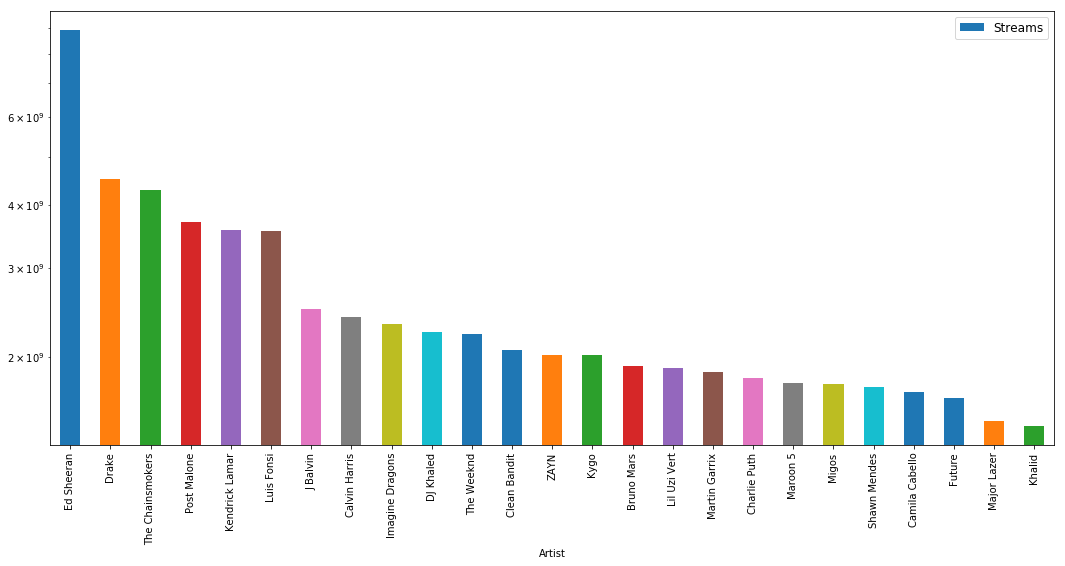
\includegraphics{output_9_0.png}
\caption{Quantidade de Streams por região}
\end{figure}

    Seguindo a mesma linha de raciocínio utilizada para ver a quantidade de
\emph{streams} por região, analisamos também a quantidade de
\emph{streams} agrupando estes por dia e por mês. Possibilitando uma
melhor análise do atributo "Streams" em amostras menores.

    \begin{Shaded}
\begin{Highlighting}[]
    \CommentTok{#Quantidade de Streams por Dia/Data}

\NormalTok{dias }\OperatorTok{=}\NormalTok{ musicas.groupby([}\StringTok{'Days'}\NormalTok{, }\StringTok{'Date'}\NormalTok{])}
\NormalTok{dias_sum }\OperatorTok{=}\NormalTok{ dias.}\BuiltInTok{sum}\NormalTok{()}

\NormalTok{dias_sum}

    \CommentTok{#Quantidade de Streams por mês}

\NormalTok{meses }\OperatorTok{=}\NormalTok{ musicas.groupby([}\StringTok{'Year'}\NormalTok{, }\StringTok{'Month'}\NormalTok{])}
\NormalTok{meses_sum }\OperatorTok{=}\NormalTok{ meses.}\BuiltInTok{sum}\NormalTok{()}
\NormalTok{meses_sum}
\end{Highlighting}
\end{Shaded}

    Com base nos agrupamentos realizados acima, pudemos gerar um gráfico
apresentando um \emph{ranking} dos cinco meses com mais \emph{streams}.

    \begin{Shaded}
\begin{Highlighting}[]
    \CommentTok{#Ranking dos 5 meses com mais Streams}

\NormalTok{meses_sum[}\StringTok{'Streams'}\NormalTok{].sort_values(ascending}\OperatorTok{=}\VariableTok{False}\NormalTok{).head().plot(kind}\OperatorTok{=}\StringTok{'bar'}\NormalTok{)}
\NormalTok{plt.rcParams[}\StringTok{'figure.figsize'}\NormalTok{] }\OperatorTok{=}\NormalTok{ (}\DecValTok{4}\NormalTok{,}\DecValTok{2}\NormalTok{)}
\NormalTok{plt.legend(loc}\OperatorTok{=}\StringTok{'upper right'}\NormalTok{, prop}\OperatorTok{=}\NormalTok{\{}\StringTok{'size'}\NormalTok{:}\DecValTok{10}\NormalTok{\}, fontsize}\OperatorTok{=}\DecValTok{5}\NormalTok{)}
\NormalTok{plt.show()}
\end{Highlighting}
\end{Shaded}

\begin{figure}
\centering
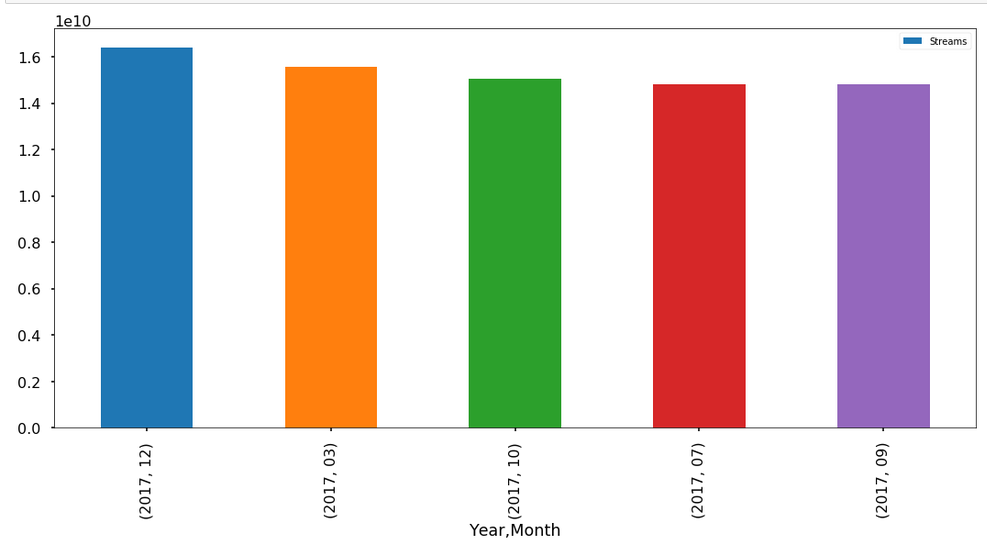
\includegraphics{StreamsPorMes.png}
\caption{Streams por Mês}
\end{figure}

    Associando a quantidade de \emph{streams} com outros atributos do
\emph{dataset}, é possível gerar outras estatísticas para análise. Após
manipularmos estas informações com base na data e região, fizemos também
a correlação entre os atributos \emph{Streams} e \emph{Artist}, e entre
os atributos \emph{Streams} e \emph{TrackName}. Limitamos a visulaização
para apenas vinte e cinco ítens e apresentamos então um \emph{ranking}
dos 25 artistas mais acessados e das 25 músicas mais acessadas,
respectivamente.

\begin{Shaded}
\begin{Highlighting}[]
\CommentTok{#Ranking dos 25 artistas mais acessados}
\NormalTok{artistas }\OperatorTok{=}\NormalTok{ musicas.groupby(}\StringTok{'Artist'}\NormalTok{)}
\NormalTok{artistas_soma }\OperatorTok{=}\NormalTok{ artistas.Streams.}\BuiltInTok{sum}\NormalTok{()}

\CommentTok{#Cria um novo dataframe para manipulação}
\NormalTok{contStreams}\OperatorTok{=}\NormalTok{pd.DataFrame(artistas_soma)}
\NormalTok{contStreamsM }\OperatorTok{=}\NormalTok{ contStreams.Streams.sort_values(ascending}\OperatorTok{=}\VariableTok{False}\NormalTok{)}
\NormalTok{contStreamsM }\OperatorTok{=}\NormalTok{ contStreamsM[:}\DecValTok{25}\NormalTok{]}

\NormalTok{contStreamsM.plot(kind}\OperatorTok{=}\StringTok{'bar'}\NormalTok{)}
\NormalTok{plt.rcParams[}\StringTok{'figure.figsize'}\NormalTok{] }\OperatorTok{=}\NormalTok{ (}\DecValTok{18}\NormalTok{,}\DecValTok{8}\NormalTok{)}
\NormalTok{plt.legend(loc}\OperatorTok{=}\StringTok{'upper right'}\NormalTok{, prop}\OperatorTok{=}\NormalTok{\{}\StringTok{'size'}\NormalTok{:}\DecValTok{12}\NormalTok{\}, fontsize}\OperatorTok{=}\DecValTok{1}\NormalTok{)}
\NormalTok{plt.yscale(}\StringTok{'log'}\NormalTok{)}
\NormalTok{plt.show()}
\end{Highlighting}
\end{Shaded}

\begin{figure}
\centering
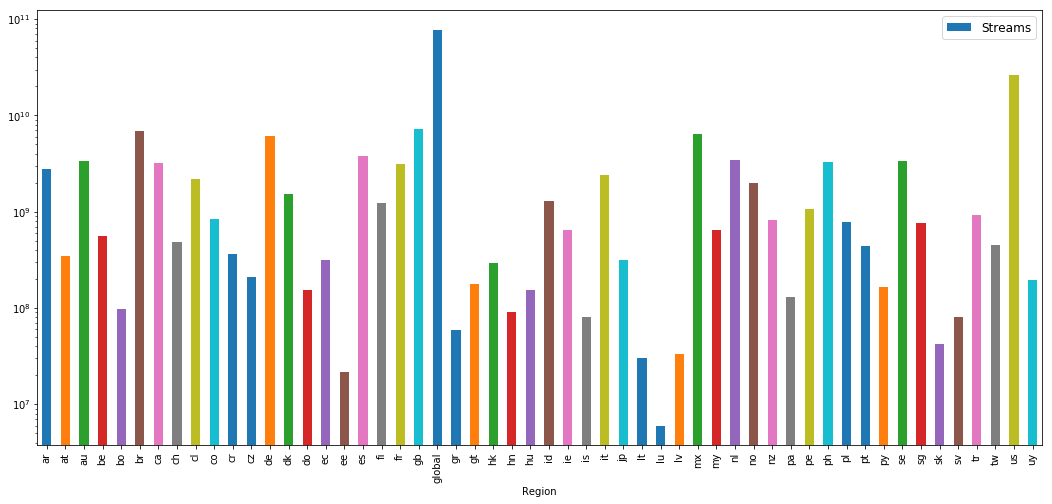
\includegraphics{output_8_0.png}
\caption{Ranking dos 25 artistas mais acessados}
\end{figure}

\begin{Shaded}
\begin{Highlighting}[]

\CommentTok{#Ranking das 25 músicas mais acessadas}
\NormalTok{musicas_mais }\OperatorTok{=}\NormalTok{ musicas.groupby(}\StringTok{'TrackName'}\NormalTok{)}
\NormalTok{musicas_mais_soma }\OperatorTok{=}\NormalTok{ musicas_mais.Streams.}\BuiltInTok{sum}\NormalTok{()}

\CommentTok{#Cria um novo dataframe para manipulação}
\NormalTok{contMusics}\OperatorTok{=}\NormalTok{pd.DataFrame(musicas_mais_soma)}
\NormalTok{contMusicsM }\OperatorTok{=}\NormalTok{ contMusics.Streams.sort_values(ascending}\OperatorTok{=}\VariableTok{False}\NormalTok{)}
\NormalTok{contMusicsM }\OperatorTok{=}\NormalTok{ contMusicsM[:}\DecValTok{25}\NormalTok{]}

\NormalTok{contMusicsM.plot(kind}\OperatorTok{=}\StringTok{'bar'}\NormalTok{)}
\NormalTok{plt.rcParams[}\StringTok{'figure.figsize'}\NormalTok{] }\OperatorTok{=}\NormalTok{ (}\DecValTok{18}\NormalTok{,}\DecValTok{8}\NormalTok{)}
\NormalTok{plt.legend(loc}\OperatorTok{=}\StringTok{'upper right'}\NormalTok{, prop}\OperatorTok{=}\NormalTok{\{}\StringTok{'size'}\NormalTok{:}\DecValTok{12}\NormalTok{\}, fontsize}\OperatorTok{=}\DecValTok{1}\NormalTok{)}
\NormalTok{plt.yscale(}\StringTok{'log'}\NormalTok{)}
\NormalTok{plt.show()}
\end{Highlighting}
\end{Shaded}

\begin{figure}
\centering
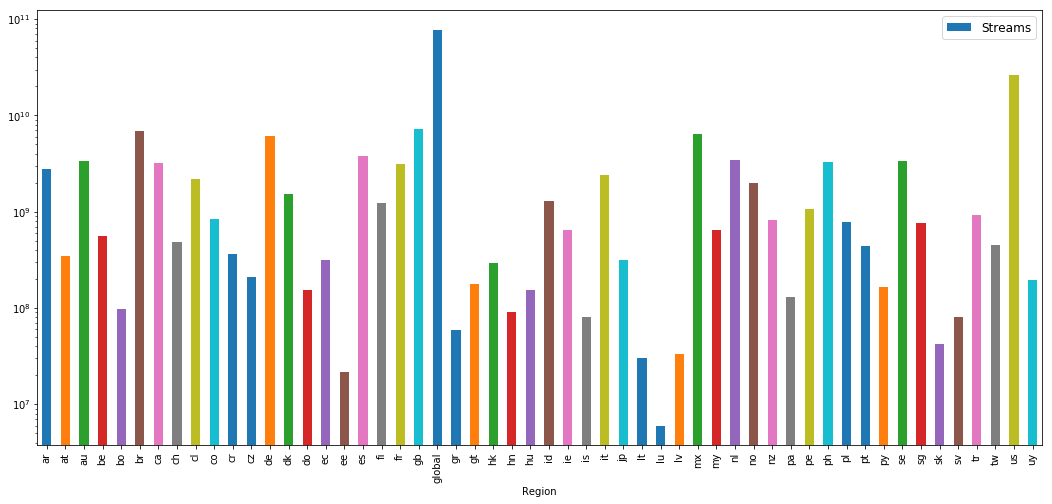
\includegraphics{output_8_0.png}
\caption{Ranking das 25 músicas mais acessados}
\end{figure}

    Em seguida foi feito um gráfico de dispersão no qual o eixo x representa
as datas e o eixo y representa as Streams. Este gráfico foi feito
pensando que, durante um ano, as visualizações de músicas podem ser mais
intensas ou não, e esta análise é interessante para, por exemplo, saber
quando colocar mais anúncios em um aplicativo por saber que o fluxo de
streams é mais intenso naquela época do ano. Ou é também para saber
quando um artista ou vários artistas lançam mais músicas e outras
análises podem ser tiradas, a partir deste gráfico, por especialistas. O
gráfico pega todas as datas presentes do nosso dataset, porém foi feita
uma filtragem dos xtickslabels, para melhorar a visualização do gráfico,
pois se não houvesse tal seleção dos xticklabels, não seria possível a
leitura das datas, tornando o gráfico ilegível.

\begin{Shaded}
\begin{Highlighting}[]
\NormalTok{fig }\OperatorTok{=}\NormalTok{ gcf()}
\NormalTok{ax }\OperatorTok{=}\NormalTok{ fig.gca()}
\NormalTok{plt.style.use(}\StringTok{'seaborn-poster'}\NormalTok{)}

\NormalTok{y }\OperatorTok{=}\NormalTok{ musicas[}\StringTok{'Streams'}\NormalTok{]}
\NormalTok{x }\OperatorTok{=}\NormalTok{ musicas[}\StringTok{'Date'}\NormalTok{] }

\NormalTok{plt.title(}\StringTok{'Streams por Data'}\NormalTok{, fontsize}\OperatorTok{=}\StringTok{'14'}\NormalTok{)}
\NormalTok{plt.xlabel(}\StringTok{'Data'}\NormalTok{, fontsize}\OperatorTok{=}\StringTok{'14'}\NormalTok{)}
\NormalTok{plt.ylabel(}\StringTok{'Streams'}\NormalTok{, fontsize}\OperatorTok{=}\StringTok{'14'}\NormalTok{)}


\CommentTok{#plt.rcParams['figure.figsize'] = (100,18)}
\CommentTok{#plt.plot(x, y ,'o',color='blue');}
\NormalTok{plt.scatter(x, y ,color}\OperatorTok{=}\StringTok{'blue'}\NormalTok{,s}\OperatorTok{=}\DecValTok{50}\NormalTok{, alpha}\OperatorTok{=}\NormalTok{.}\DecValTok{5}\NormalTok{ )}\OperatorTok{;}

\NormalTok{xmarks}\OperatorTok{=}\NormalTok{[}\StringTok{'2017-01-01'}\NormalTok{,}\StringTok{'2017-03-18'}\NormalTok{,}\StringTok{'2017-08-30'}\NormalTok{,}\StringTok{'2018-01-09'}\NormalTok{] }\CommentTok{# 5 registros}
\NormalTok{plt.xticks(xmarks)}

\NormalTok{labels }\OperatorTok{=}\NormalTok{ [item.get_text() }\ControlFlowTok{for}\NormalTok{ item }\KeywordTok{in}\NormalTok{ ax.get_xticklabels()]}
\NormalTok{labels[}\DecValTok{0}\NormalTok{] }\OperatorTok{=} \StringTok{'2017-01-01'}
\NormalTok{labels[}\DecValTok{1}\NormalTok{] }\OperatorTok{=} \StringTok{'2017-03-18'}
\NormalTok{labels[}\DecValTok{2}\NormalTok{] }\OperatorTok{=} \StringTok{'2017-08-30'}
\NormalTok{labels[}\DecValTok{3}\NormalTok{] }\OperatorTok{=} \StringTok{'2018-01-09'}
\NormalTok{ax.set_xticklabels(labels)}

\NormalTok{plt.savefig(}\StringTok{'StreamsPorData.png'}\NormalTok{) }
\end{Highlighting}
\end{Shaded}

\begin{figure}
\centering
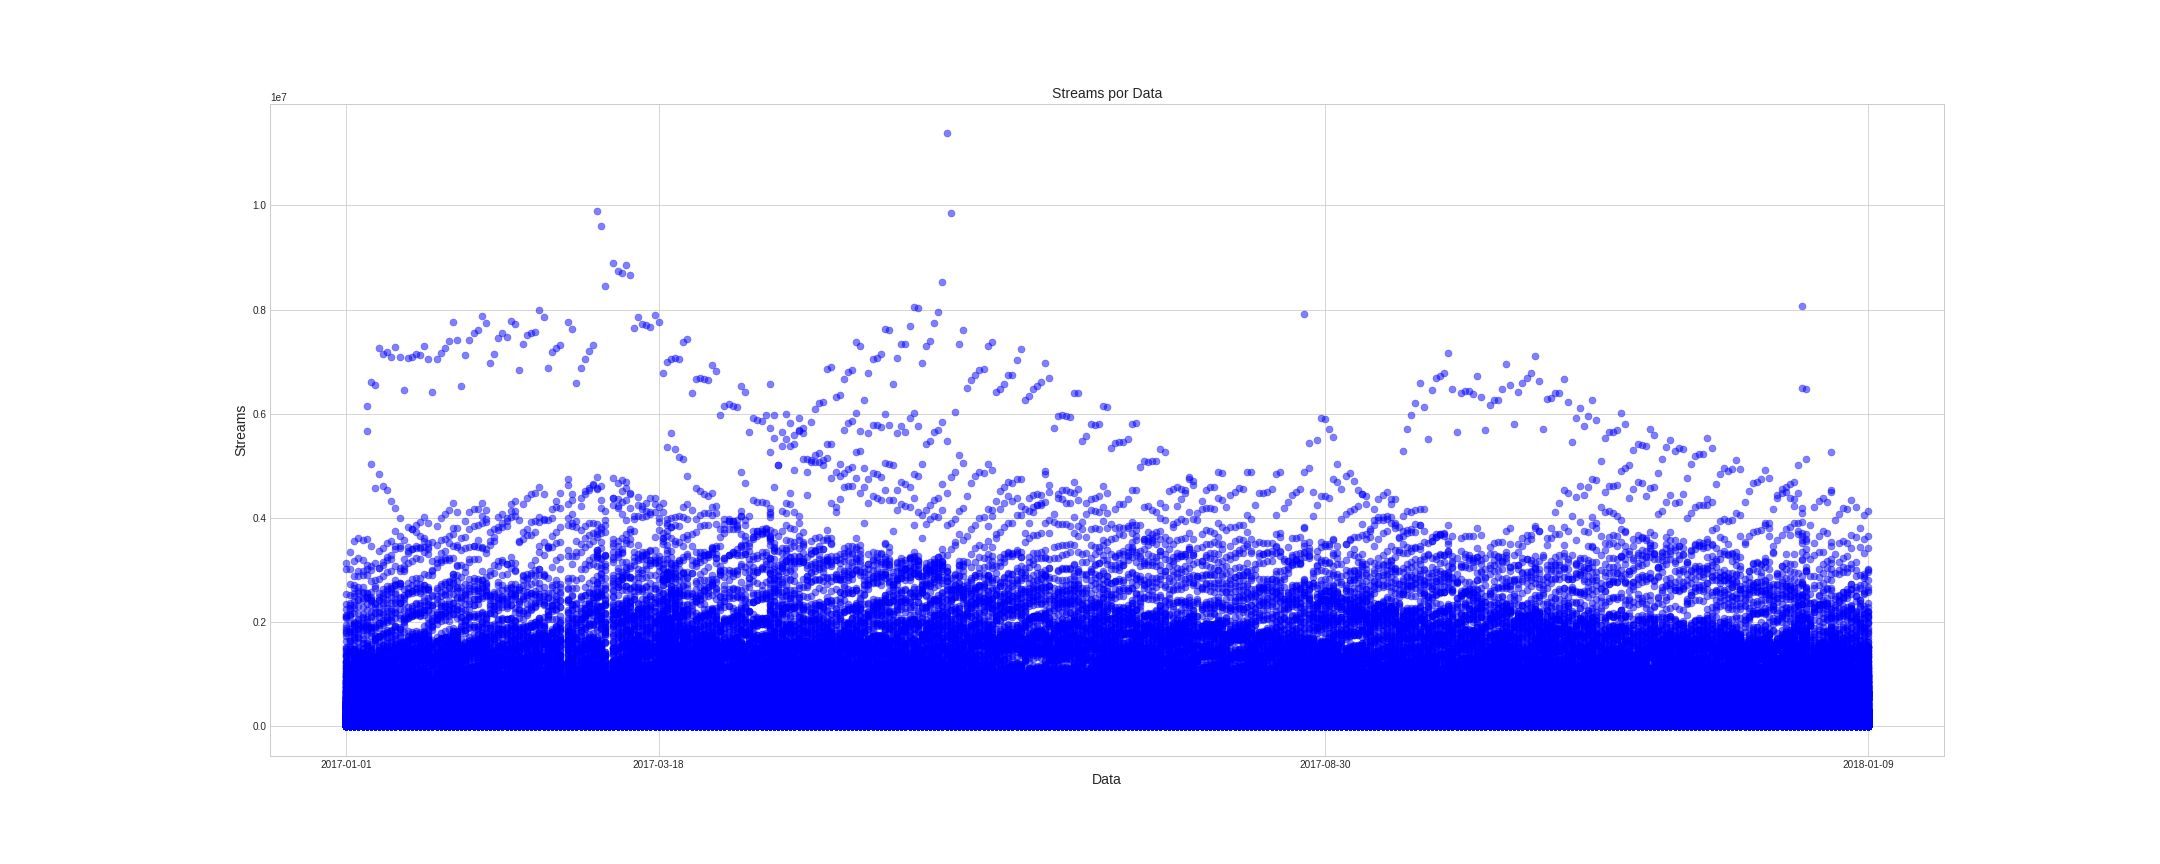
\includegraphics{StreamsPorData.png}
\caption{Gráfico de Dispersão - Streams por Data}
\end{figure}

    Foi feito também um outro gráfico de dispersão, no qual o eixo x
representa o nome do cantor e o eixo y representa a track name, que
seria o nome da música, sendo assim, gera uma relação que representa a
música de cada cantor. Além disso foi representada uma outra camada de
cor, através de um colorbar, que representa as Streamns, dessa forma,
mostra para nós uma análise das músicas mais tocadas de cada cantor.
Essa análise é muito interessante pois se rodada com o dataset inteiro
mostraria todas as músicas mais tocadas de todos os cantores.

\begin{Shaded}
\begin{Highlighting}[]

\CommentTok{#Ranking dos 50 musicas mais acessadas, com seus artistas}
\NormalTok{artistas_mus }\OperatorTok{=}\NormalTok{ musicas.groupby([}\StringTok{'Artist'}\NormalTok{, }\StringTok{'TrackName'}\NormalTok{])}
\NormalTok{artistas_mus }\OperatorTok{=}\NormalTok{ artistas_mus.Streams.}\BuiltInTok{sum}\NormalTok{()}
\NormalTok{artistas_mus}
\CommentTok{#Cria um novo dataframe para manipulação}
\NormalTok{artistas_musf}\OperatorTok{=}\NormalTok{pd.DataFrame(artistas_mus)}
\NormalTok{artistas_musf }\OperatorTok{=}\NormalTok{ artistas_musf.Streams.sort_values(ascending}\OperatorTok{=}\VariableTok{False}\NormalTok{)}
\NormalTok{artistas_musf }\OperatorTok{=}\NormalTok{ artistas_musf[:}\DecValTok{50}\NormalTok{]}
\NormalTok{art }\OperatorTok{=}\NormalTok{ artistas_musf.reset_index()}
\NormalTok{art}

\NormalTok{fig }\OperatorTok{=}\NormalTok{ gcf()}
\NormalTok{ax }\OperatorTok{=}\NormalTok{ fig.gca()}
\NormalTok{plt.style.use(}\StringTok{'seaborn-poster'}\NormalTok{)}

\NormalTok{X }\OperatorTok{=}\NormalTok{ art[}\StringTok{'Artist'}\NormalTok{]}
\NormalTok{Y }\OperatorTok{=}\NormalTok{ art[}\StringTok{'TrackName'}\NormalTok{]}
\NormalTok{C }\OperatorTok{=}\NormalTok{ art[}\StringTok{'Streams'}\NormalTok{]}

\NormalTok{plt.rcParams[}\StringTok{'figure.figsize'}\NormalTok{] }\OperatorTok{=}\NormalTok{ (}\DecValTok{100}\NormalTok{,}\DecValTok{50}\NormalTok{)}

\CommentTok{#cmap = mpl.colors.ListedColormap([ 'tab:red', 'tab:orange',  'tab:red'])}


\NormalTok{s }\OperatorTok{=}\NormalTok{ ax.scatter(X,Y,c}\OperatorTok{=}\NormalTok{C,lw}\OperatorTok{=}\FloatTok{0.3}\NormalTok{, s}\OperatorTok{=}\DecValTok{500}\NormalTok{, alpha}\OperatorTok{=}\FloatTok{0.5}\NormalTok{,  cmap}\OperatorTok{=}\StringTok{'autumn'}\NormalTok{) }\CommentTok{#plasma,hsv  'viridis', 'plasma', 'inferno', 'magma', 'cividis', 'autumn']}

\NormalTok{plt.title(}\StringTok{'Gráfico de artistas por Track name em função das streams.'}\NormalTok{, fontsize}\OperatorTok{=}\StringTok{'22'}\NormalTok{)}
\NormalTok{plt.ylabel(}\StringTok{'Track Name'}\NormalTok{, fontsize}\OperatorTok{=}\StringTok{'14'}\NormalTok{)}
\NormalTok{plt.xlabel(}\StringTok{'Artist'}\NormalTok{, fontsize}\OperatorTok{=}\StringTok{'14'}\NormalTok{)}


\CommentTok{#norm = mpl.colors.Normalize(vmin=1, vmax=20)}
\NormalTok{cb }\OperatorTok{=}\NormalTok{ plt.colorbar(s)}

\NormalTok{cb.set_label(}\StringTok{'Streams'}\NormalTok{, fontsize}\OperatorTok{=}\StringTok{'14'}\NormalTok{)}


\NormalTok{plt.savefig(}\StringTok{'ArtistasPorStreamsCores.png'}\NormalTok{) }
\end{Highlighting}
\end{Shaded}

\begin{figure}
\centering
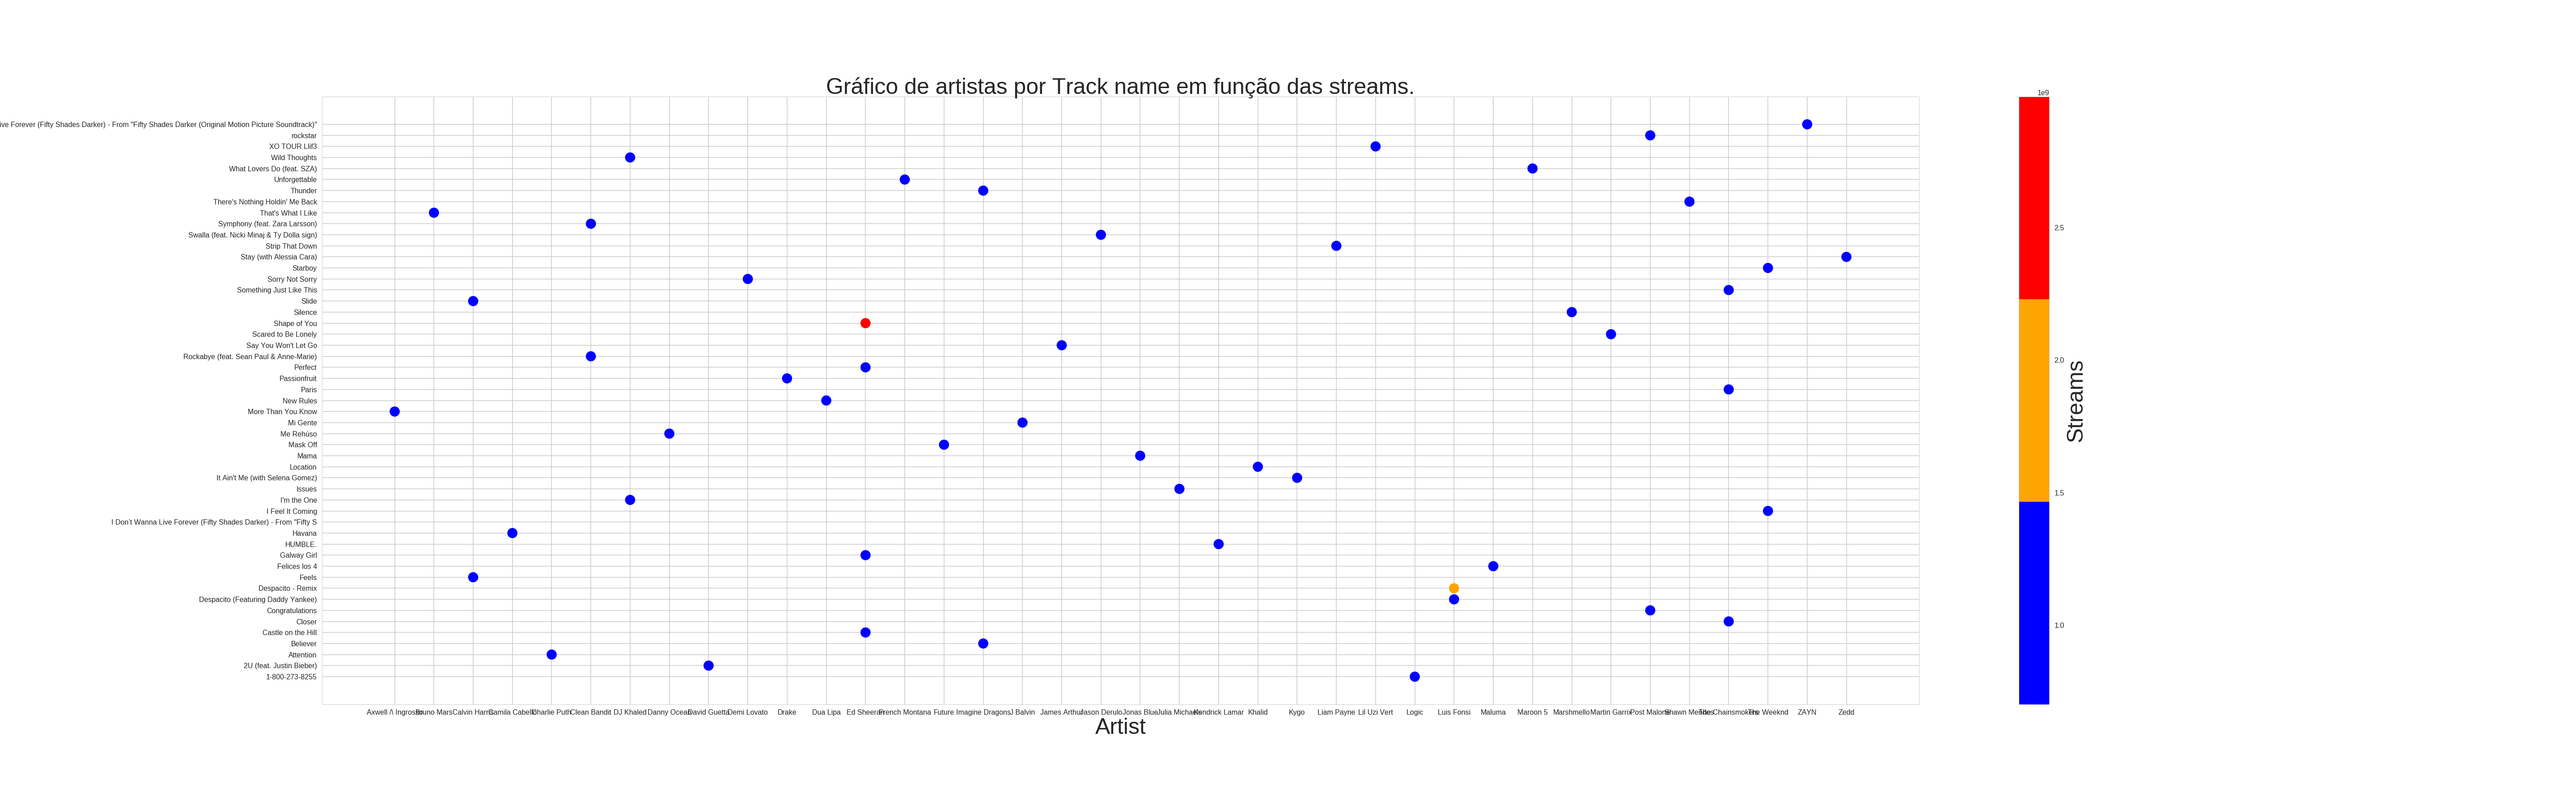
\includegraphics{ArtistasPorStreamsCores.png}
\caption{Gráfico de Dispersão - Artistas por Streams}
\end{figure}


    % Add a bibliography block to the postdoc
    
    
    
    \end{document}
